\documentclass[conference]{IEEEtran}

  	\usepackage[pdftex]{graphicx}
  	\graphicspath{{../pdf/}{../jpeg/}}
	\DeclareGraphicsExtensions{.pdf,.jpeg,.png}

	\usepackage[cmex10]{amsmath}
	\usepackage{mathabx}
	\usepackage{algorithmic}
	\usepackage{array}
	\usepackage{mdwmath}
	\usepackage{mdwtab}
	\usepackage{eqparbox}
	\usepackage{url}
    \usepackage[numbers,sort&compress]{natbib}
	\hyphenation{op-tical net-works semi-conduc-tor}

\setlength{\parskip}{1em}
\renewcommand{\baselinestretch}{1.0}
\thispagestyle{plain}
\pagestyle{plain}

\begin{document}


% =========
% # TITLE #
% =========

\title{\LARGE An SVN model-based approach to assessing the gap between strategy and implementation: The case of Kashiwa-no-ha Smart City}

% ==========
% # AUTHOR #
% ==========

% \author{\authorblockN{Leave Author List blank for your IMS2013 Summary (initial) submission.\\ IMS2013 will be rigorously enforcing the new double-blind reviewing requirements.}
% \authorblockA{\authorrefmark{1}Leave Affiliation List blank for your Summary (initial) submission}}

 \author{\authorblockN{
 Maya F. Dhondt\authorrefmark{1}, 
 Yulong Wang\authorrefmark{1}, 
 Giles B. Sioen\authorrefmark{2},
 Aigerim Shopenova \authorrefmark{1},
 Motoharu Onuki\authorrefmark{1}, and 
 Takashi Mino\authorrefmark{1}
 }
 \authorblockA{
Graduate Program in Sustainability Science - Global Leadership Initiative (GPSS-GLI)\\
The University of Tokyo, Kashiwa, Japan
 \authorrefmark{1}\\ 
 maya.dhondt@s.k.u-tokyo.ac.jp\authorrefmark{1} 
 %yulong.wang@s.k.u-tokyo.ac.jp\authorrefmark{1}
 }
 \authorblockA{
Department of Human and Engineered Environmental Studies\\
The University of Tokyo, Kashiwa, Japan
 \authorrefmark{2}\\ 
 gilessioen@edu.k.u-tokyo.ac.jp\authorrefmark{2}
 }}

\maketitle

% ============
% # ABSTRACT #
% ============

\begin{abstract}
Smart city creation emphasizes technological advancements, but social aspects must be equally considered for sustainable development. In Kashiwa-no-ha Smart City, located in Chiba, Japan, focus is given to stakeholder collaboration to achieve the project's goals. This strategy is implemented through the creation of the Urban Design Center Kashiwa-no-ha (UDCK), a platform for the public-private-academic partnership that leads the smart city project. However, socio-technical problems emerging in the area show that implementation of UDCK has not been able to ensure both social and technological issues have been adequately considered.
In this paper, we employed a Stakeholder Value Network (SVN) model to reveal relationships between stakeholders and understand ways in which the smart city strategy implementation could be improved. The SVN showed that UDCK's potential as a facilitator for stakeholder collaboration has not been fully realized. In recent years, transdisciplinary concepts like the ``living lab'' which empower service users to be involved in decision-making processes have been presented as a better means to tackle complex problems and create value. We proposed that by adopting a transdisciplinary approach and improving feedback processes from beneficiaries (residents, businesses, and incubators) to service providers (public-private-academic partnership), this gap between strategy and implementation could be addressed.
\end{abstract}

% ============
% # KEYWORDS #
% ============

\IEEEoverridecommandlockouts
\begin{keywords}
Stakeholder value network, stakeholder education, smart city, transdisciplinary science.
\end{keywords}
\IEEEpeerreviewmaketitle

% ===================
% # I. Introduction #
% ===================

\section{\textbf{Introduction}}

Cities are developed for people, however, existing literature on smart cities has emphasized technological advancements \cite{nam2011smart}. While social elements have also been elaborated on in discussing the characteristics and activities of ``smart'' citizens \cite{giffinger2007smart}, there is a need to address socio-technical issues holistically \cite{zubizarreta2015smart}. This can allow computing technologies to be developed specifically for living activities \cite{washburn2009helping}, rather than focusing on technology alone \cite{fernandez2016stakeholders}. In Japan, governments and developers are working together for the development of smart cities while focusing on culture, science \cite{keihanna}, transportation, the reduction of energy use \citep{toyota,future}, and even health and wellbeing \cite{trencher2017stretching}.

Collaborations between stakeholders can foster sustainable city development. One way for this to take place is by the establishment of a mediator that helps to facilitate collaboration among stakeholders. This is the case in Kashiwa-no-ha, a smart city located in Chiba Prefecture, Japan, with a population of 11,552 \cite{kashiwa}. Kashiwa-no-ha Smart City is planned to become an environmental-symbiotic city of new industry creation, health, and longevity. To achieve this goal, it utilizes extensive stakeholder collaboration with public-private-academic partners, which is given physical form by the Urban Design Center Kashiwa-no-ha (UDCK).

UDCK has implemented different types of activities in response to the diverse needs of stakeholders and multiple goals of the city: (1) research collaboration between universities, businesses, and residents, (2) connecting technology to residents’' lives, (3) collaborative management of urban spaces, (4) provision of community activity opportunities. However, despite the establishment of UDCK as a cornerstone of the smart city strategy for stakeholder engagement and planning coordination, newly emerging socio-technical problems counter to the project’s goals can be found.

These problems are diverse. Some are problems many cities are facing (such as Japan's rapidly shrinking and aging society), and some are more unique to the specific situation of Kashiwa-no-ha (such as a lack of cultural identity within the newly developed area). These problems have a high level of complexity, with many different stakeholder involvements. In order to understand and solve these individual problems, an in-depth understanding of stakeholder relationships is required. To achieve this, the creation of a Stakeholder Value Network (SVN) to model the stakeholder associations is useful.

The emergence of these problems within Kashiwa-no-ha demonstrates that although UDCK has been established as part of the strategy to achieve the smart city goals, implementation has been challenging. With the use of SVN, this paper intends to discover discrepancies between the smart city strategy and implementation that allow problems counter to the smart city goals to become evident. The use of systems thinking in urban planning has been successfully used for this purpose in previous studies \citep{mino2016philosophy,webb2018sustainable,street2015cost}.


% =======================
% # II. Research design #
% =======================

\section{\textbf{Research design}}

This paper aims to frame newly emerging socio-technical problems in Kashiwa-no-ha to improve the services from and for the stakeholders identified during a previous stage of this research. Given the emergence of these problems, the analysis aims to understand areas requiring improvement in the implementation of the smart city strategy and uncover ways to address these gaps. To reach this aim, two steps are developed as follows: (1) SVN analysis is conducted to identify areas of ineffective strategy implementation, and (2) based on the previous step, suggestions are made to solve this problem.

\subsection{\textbf{Methodology}}

\subsubsection{\textbf{Introduction}}\

\
This research was developed based on the results of a Global Field Exercise (GFE) at the Graduate Program in Sustainability Science – Global Leadership Initiative (GPSS-GLI), part of the Graduate School of Frontier Sciences (GSFS), The University of Tokyo. GFEs are field-oriented exercises organized in a variety of study areas, implemented by GPSS-GLI to offer students the opportunity to develop fieldwork competencies, including group work activities and discussions with stakeholders \cite{chan2004systems}. The GFE upon which the results presented within this research are based focused on finding solutions to newly emerging problems in Kashiwa-no-ha Smart City.

A site visit was held on Oct. 31, 2017, and stakeholder meetings between Nov. 2017 and Dec. 2017 with the city government, UDCK, and the developers. To ensure a better understanding of the complexity of the case, five teams of 5-6 students identified newly emerging socio-technical problems in the case study in collaboration with the above-mentioned stakeholders. The problems were categorized according to social importance and linkages with the smart city goals within their corresponding problem space \cite{de2011engineering}. The problems identified were: (1) unresilient energy supply from traditional sources (e.g. fossil fuel based), (2) lack of cultural identity, (3) difficulties in creating an enterprise mix for economic resilience, (4) lack of quality of life of international residents, (5) population decline and lack of inbound migration.

Given the wide range of problems identified by the five teams, data was collected from a number of different sources. Literature review was completed by each team to provide context for smart city projects and the socio-technical problems identified. Secondary data was documented to set out background for the case study area with existing data. Questionnaire surveys (4), stakeholder interviews (8), and a focus group discussion (1) were conducted by the different teams to gain an understanding of stakeholder viewpoints and relationships. Questionnaire surveys (1) and (2) targeted 50 startup members of 2 local business incubators, with 4 responses for each. Questionnaire survey (3) targeted 280 residents and received 54 responses. Questionnaire survey (4) targeted the international students of The University of Tokyo Kashiwa Campus in 2 rounds, with 55 and 40 responses respectively. Stakeholder interviews were made with representatives of city government (1), the developers (1), residents (1), business (4) and academia (1). The focus group discussion was conducted with 3 older residents.

Having collected data within separate teams, the underlying cause of the socio-technical problems was then examined in the next step collaboratively.

\subsubsection{\textbf{Stakeholder Value Network}}\

\
SVN is a modeling approach which can be used to understand the impacts of relationships between project stakeholders and the success of the project \cite{feng2010dependency}. The relationships between Kashiwa-no-ha Smart City stakeholders and the services they provide were documented in an SVN. This was done to reveal value flows between stakeholders and  examine whether the underlying cause of the emerging socio-technical problems identified could be determined. The data was obtained in in the previous step of the research by the individual teams. Collaboration amongst the groups was facilitated by one coordinator and a representative of each team to combine the data they had derived. The primary roles of service participants were clustered and characterized as distinct stakeholders within the value flow network. Stakeholders are connected through creation and consumption of value categorized as (1) services, (2) business services, (3) policy, and (4) finance.

Based on this, weaknesses in the SVN could be identified for better understanding of the efficacy of the smart city strategy and potential for improvement in the implementation of it. 


% ================
% # III. Results #
% ================

\section{\textbf{Results}}

\subsection{\textbf{Results of SVN analysis}}

The identified socio-technical problems were described in relation to their corresponding stakeholders (Table 1).

\begin{table}[ht!] %!t
\centering
\caption{Summary of stakeholder groups of Kashiwa-no-ha Smart City identified as part of SVN analysis.}
\begin{tabular}{|c|c|p{2in}|}
 \hline
\bfseries No.&\bfseries  Stakeholder&\bfseries Description\\
 \hline
1& UDCK & Public-private-academic partnership between stakeholders 2-4 (Kashiwa city government, The University of Tokyo, and Mitsui Fudosan) \\
 \hline
2& Government & Including stakeholder sub-groups: local (Kashiwa city), prefectural (Chiba prefecture), and national (Japan) \\
 \hline
3& Academia & i.e. local universities and their members (including The University of Tokyo, Chiba University, etc.) \\
 \hline
4& Developers & i.e. Mitsui Fudosan, a private real estate development company \\
 \hline
5& Residents & Including (but not limited to) stakeholder sub-groups: older residents, international residents \\
 \hline
6& Visitors & N/A \\
 \hline
7& Business & Including (but not limited to) stakeholder sub-groups: entrepreneurs, startups, companies and employees \\
 \hline
8& Incubators & i.e. KOIL (a startup incubator affiliated with private real estate developers Mitsui Fudosan), Todai Kashiwa Venture Plaza (an academic startup incubator affiliated with The University of Tokyo), and Tokatsu Techno Plaza (a business incubator affiliated with Kashiwa City and the University of Tokyo) \\
 \hline
\end{tabular}
\label{TABLE}
\end{table}

\textbf{UDCK:} UDCK provides a platform for the public-private-academic partnership to implement strategy in Kashiwa-no-ha Smart City.

\textbf{Government:} The role of the local government in the development of Kashiwa-no-ha Smart City is mainly to provide public services, such as daily services (e.g. sanitation, energy, and public safety; infrastructure services; and policy services) through regulation of other stakeholders. The role this stakeholder plays differs among smart cities. For example, government plays a larger investment role in South America, resulting in proliferation of smart cities in the area. In European countries, local governments enable small and medium-sized cities to collaborate and function as a single big city \cite{claudel2015government}. In Japan, due to severe financial constraints in all levels of government, the development strategy of Kashiwa-no-ha Smart City relies more on collaboration with academia and private developers.

Under the coordination of a platform like UDCK, Kashiwa-no-ha has been able to implement initiatives. For example, a stormwater retention pond is located in the middle of the smart city. As its function is to ensure water regulation in the area, development of the pond was forbidden. Public access to the area was limited, and it was an unattractive area in a central location. However, with the support of local government, a middle-ground solution was reached. While technical function of the retention pond had to be guaranteed, local government gave permission for the area to be redesigned to create an attractive ``aqua terrace'', opened to the public in Nov. 2016 \cite{mitsui}.

\textbf{Academia:} In the Kashiwa-no-ha Smart City, academic institutions play a very important role. This is not only because there are a large number of employees and students in the universities (who are reliant on services provided by other stakeholder groups), but because these academic institutions provide services in the smart city, many of which are coordinated by UDCK. The University of Tokyo facilitates an Urban Design Studio course. In the studio, students present an image for the future of Kashiwa through open discussion with government, business, and residents. Some of these proposals have been implemented as UDCK projects in the area. However, while the University of Tokyo has placed a lot of effort into the creation of such experiments, initiatives have often been implemented only for the duration of the initial funding period, disappearing soon after. For example, Intelligent Transportation Systems (ITS) (which included, for example, bicycle and car sharing schemes) were put into effect in Kashiwa-no-ha in 2007, but were later discontinued \cite{kashiwanoha}.

\textbf{Developers:} As a company that has been associated with the Kashiwa region for more than 140 years, Mitsui Fudosan has been the main real estate developers of Kashiwa-no-ha Smart City. While primarily providing infrastructure, Mitsui Fudosan has also made various other contributions to Kashiwa-no-ha Smart City. These include living services and entertainment facilities: the first project of Kashiwa-no-ha Smart City was the development of the compact shopping mall LaLaport Kashiwa-no-ha, which provides services through nearly 200 retail stores, restaurants and companies providing services. After the Great East Japan Earthquake, Mitsui Fudosan implemented a city-scale ``Disaster Ready Energy System'' to ensure the continued provision of (limited) electricity to public areas in emergencies in order to ensure the continuation of services and prevent threats to life and economic losses. However, despite the implementation of smart grid technology, the energy system remains heavily reliant on traditional fossil fuel sources.

\textbf{Residents:} Residents are the main recipients of various services in smart cities. In Kashiwa-no-ha Smart City, many residents also participate in a number of UDCK and academia-implemented experiments, such as the above-mentioned bike and car sharing schemes. There is a rare opportunity for such experiments within Kashiwa-no-ha as the residents have characteristics that differentiate them from residents of other areas: high internationalization, wide range of age groups, and many have relocated after (and especially for) the establishment of the smart city.

\textbf{Visitors:} Payments by visitors for services and taxes generated from purchases are important income sources for Kashiwa-no-ha Smart City. In fact, attracting tourists is one of the development strategies of the smart city. From the perspective of systems thinking, visitors are external elements of the smart city system, however, they are the best evidence of the attractiveness of Kashiwa-no-ha - frequent visits bring vitality to the economy. Additionally, visitors have potential to be attracted as migrants and become permanent residents of the smart city.

\textbf{Business:} Businesses provide many services within the smart city, contributing to economic robustness and generating employment in the area. Attracting a diverse mix of enterprise models and industry types to the city is part of the strategy of Kashiwa-no-ha Smart City, but this is an ongoing goal. To attract businesses to Kashiwa-no-ha, stakeholders provide services marketed to businesses. These key pulls are (1) proximity to academia (for research and development services), (2) the ability to test innovations with the population who have an interest in smart city concepts and inventive ideas, and (3) infrastructure (especially in the form of business incubators).

\textbf{Incubators:} In order to achieve the aim of a diverse mix of enterprise models, a number of startup incubators are in operation in Kashiwa-no-ha. Developers Mitsui Fudosan have opened Kashiwa-no-ha Open Innovation Lab (KOIL) as an incubator offering infrastructure and business support to 38 local startups and 230 individual entrepreneurs. The University of Tokyo (with the support of local government and other local universities such as Chiba University), provides a platform for startups to be developed from research initiatives and for established businesses to obtain research and development services through incubators: Todai Kashiwa Venture Plaza and Tokatsu Techno Plaza have 17 startup and 34 startup and SME members respectively.


Based on earlier stakeholder interviews and collaboration of representatives from each of the five teams, the SVN was created (Fig. 1). It was found that some stakeholders were overrepresented, while others exerted little influence in the determination of value flows. UDCK has, despite its presence as a platform for public-private-academic partnership, limited promotion and lack of accessibility to other stakeholders, especially residents. However, residents are intended to be the main beneficiaries of the collaboration. Consequently, this has led to the underutilization of UDCK’s potential. At present, the smart city value is not fully reflected as some socio-technical issues uncovered in this research have not yet been considered by the stakeholders (e.g. population decline, and a lack of cultural identity).

\begin{figure}[ht!] %!t
\centering
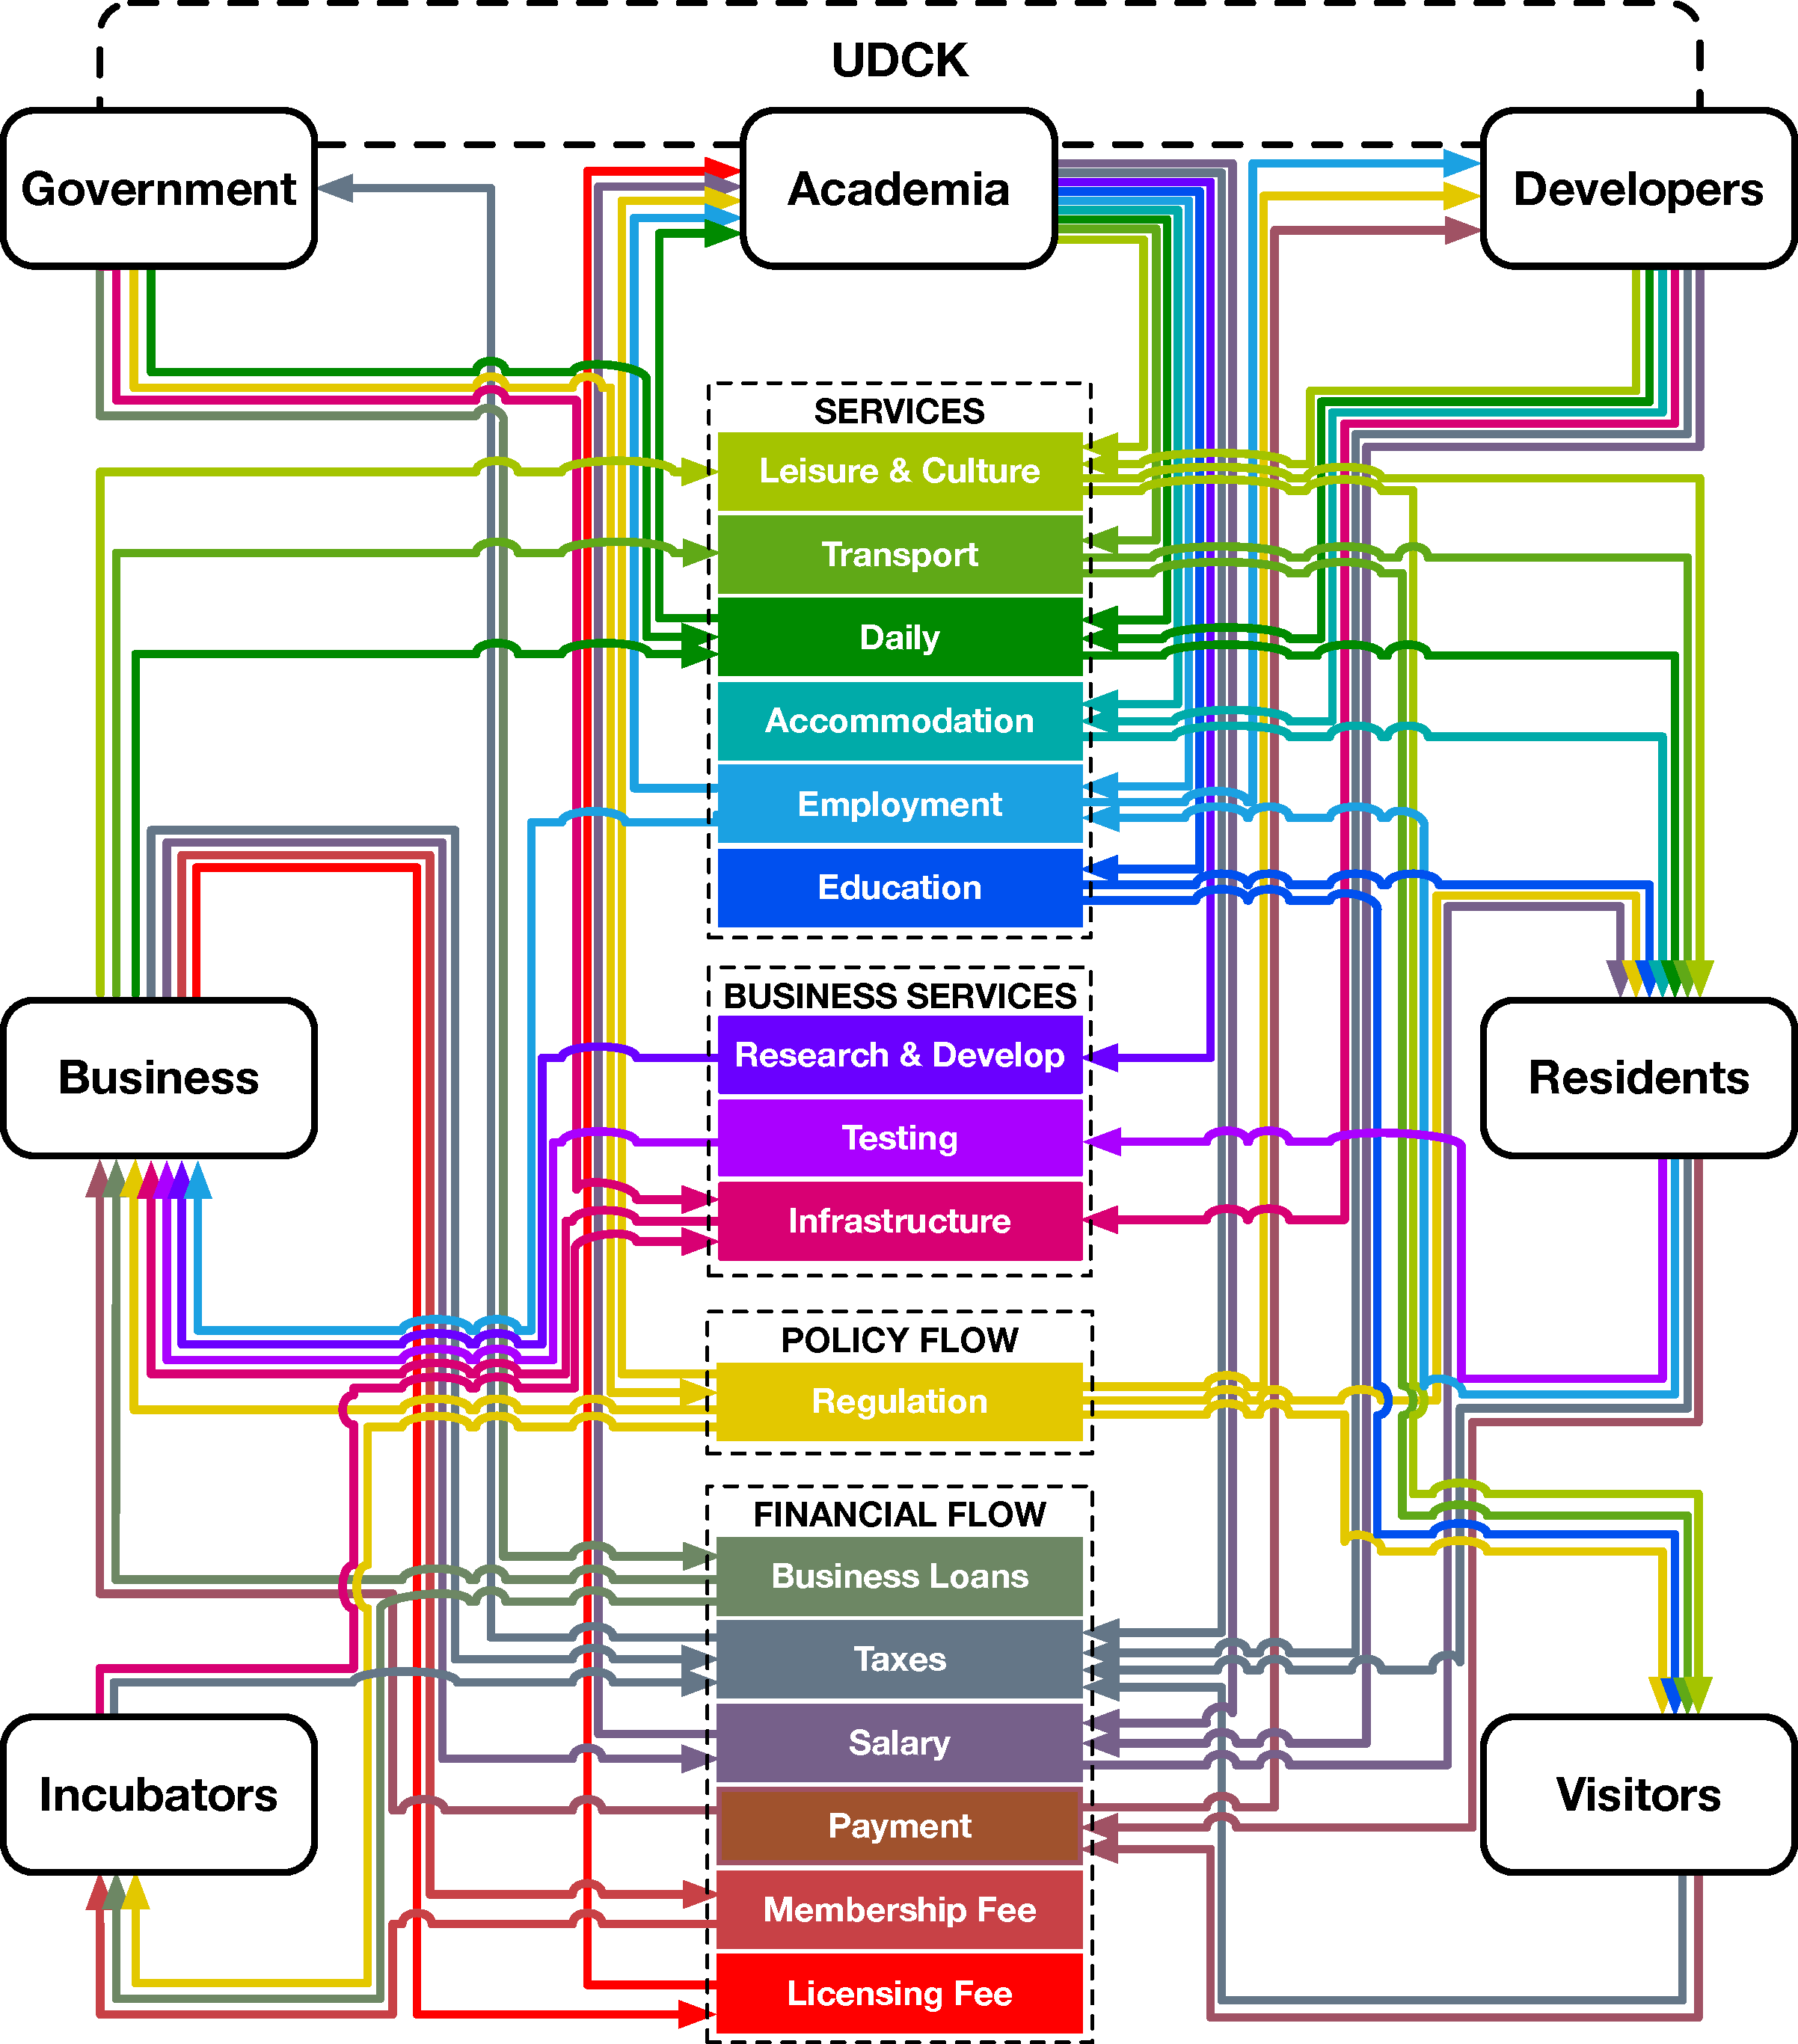
\includegraphics[width=3.5in]{SVN_1_v_7.pdf}
\caption{SVN for stakeholders of the Kashiwa-no-ha Smart City.}
\label{FULL}
\end{figure}

\subsection{\textbf{Improving the strategy}}

\
Recent literature describes transdisciplinary approaches, in which projects are co-designed with all stakeholders and especially beneficiaries (i.e. residents), to avoid top-down decision-making \cite{jerneck2011structuring}. This approach serves to bridge both aspects of socio-technical problems by integrating society's needs \cite{lang2012transdisciplinary}. This decision-making power is represented in the regulation flow in the SVN (Fig. 2). The current situation leads to a lack of interpretation of the beneficiaries needs as depicted in Fig. 2.

\begin{figure}[ht!] %!t
\centering
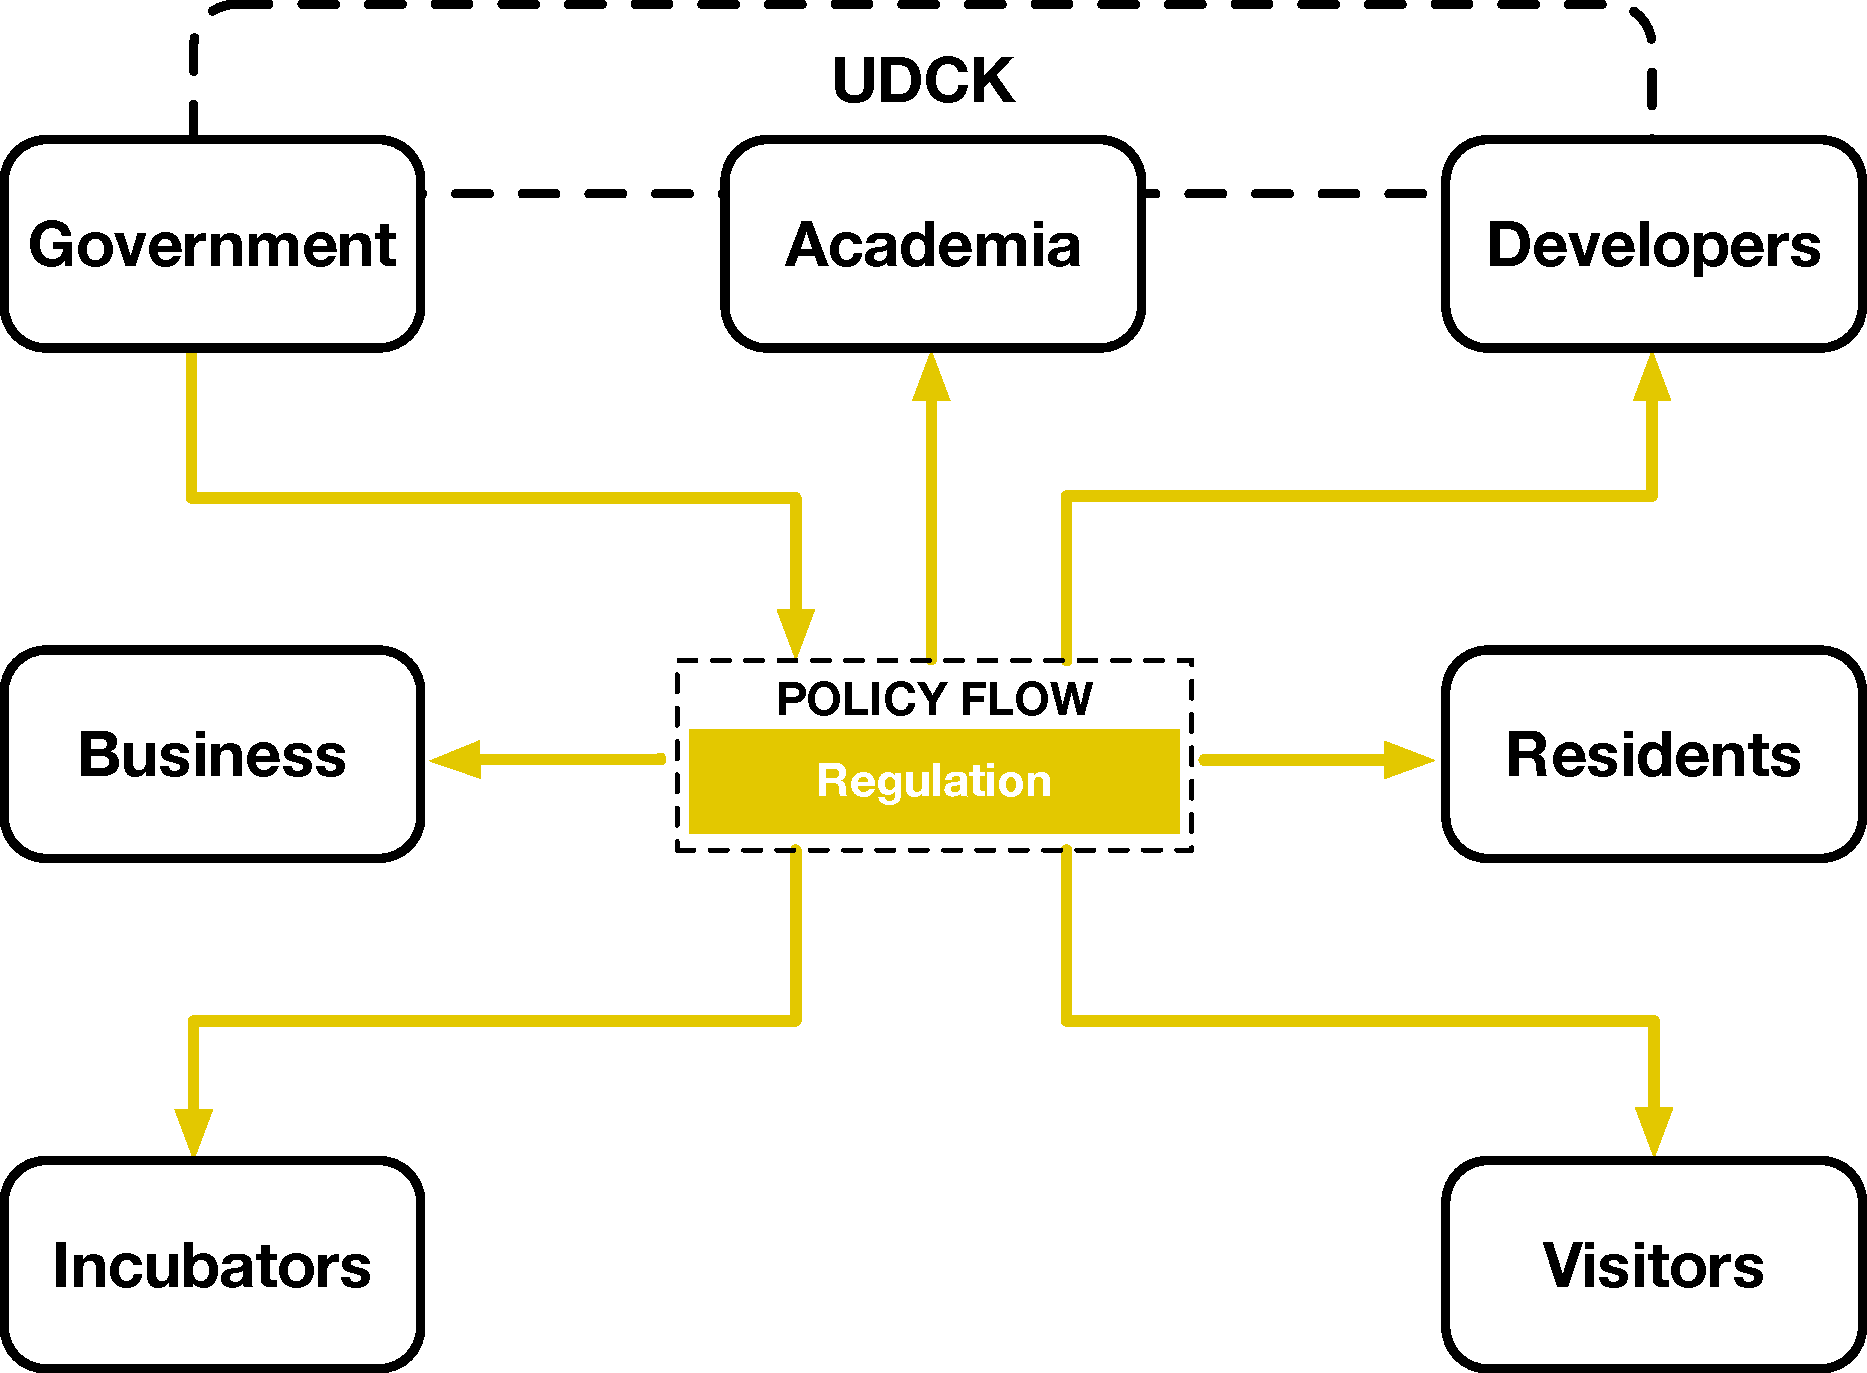
\includegraphics[width=2.5in]{SVN_2_v_6.pdf}
\caption{SVN for stakeholders of the Kashiwa-no-ha Smart City: regulation value flows only.}
\label{REGULATION}
\end{figure}

In the Kashiwa-no-ha Smart City system, the public-private-academic partners work together in the coordination of UDCK. This includes complex policy implementation processes with many stakeholders and beneficiaries involved. Currently, residents feel that strategy in Kashiwa-no-ha is implemented without consideration of their voices.

Considering this, the SVN was modified to empower residents, local businesses, and incubators to be involved in the decisions of UDCK, with regulation value flowing from these stakeholders to government added (Fig. 3). With this feedback, residents, business, and incubators can influence UDCK, which can in turn provide better services through the public-private-academic partnership.

This can be realized by involving stakeholders in decision-making. For instance, as the smart city strategy involves attracting a wide range of enterprise models to Kashiwa-no-ha, by including business stakeholders in strategy decisions, the likelihood of strategy success increased. For example, business has stated that a lack of venture capital in Kashiwa-no-ha is the reason that startup business in certain sectors has not seen success in the area. By considering these kinds of viewpoints, the development team could focus their strategy to tackle these issues.

\begin{figure}[ht!] %!t
\centering
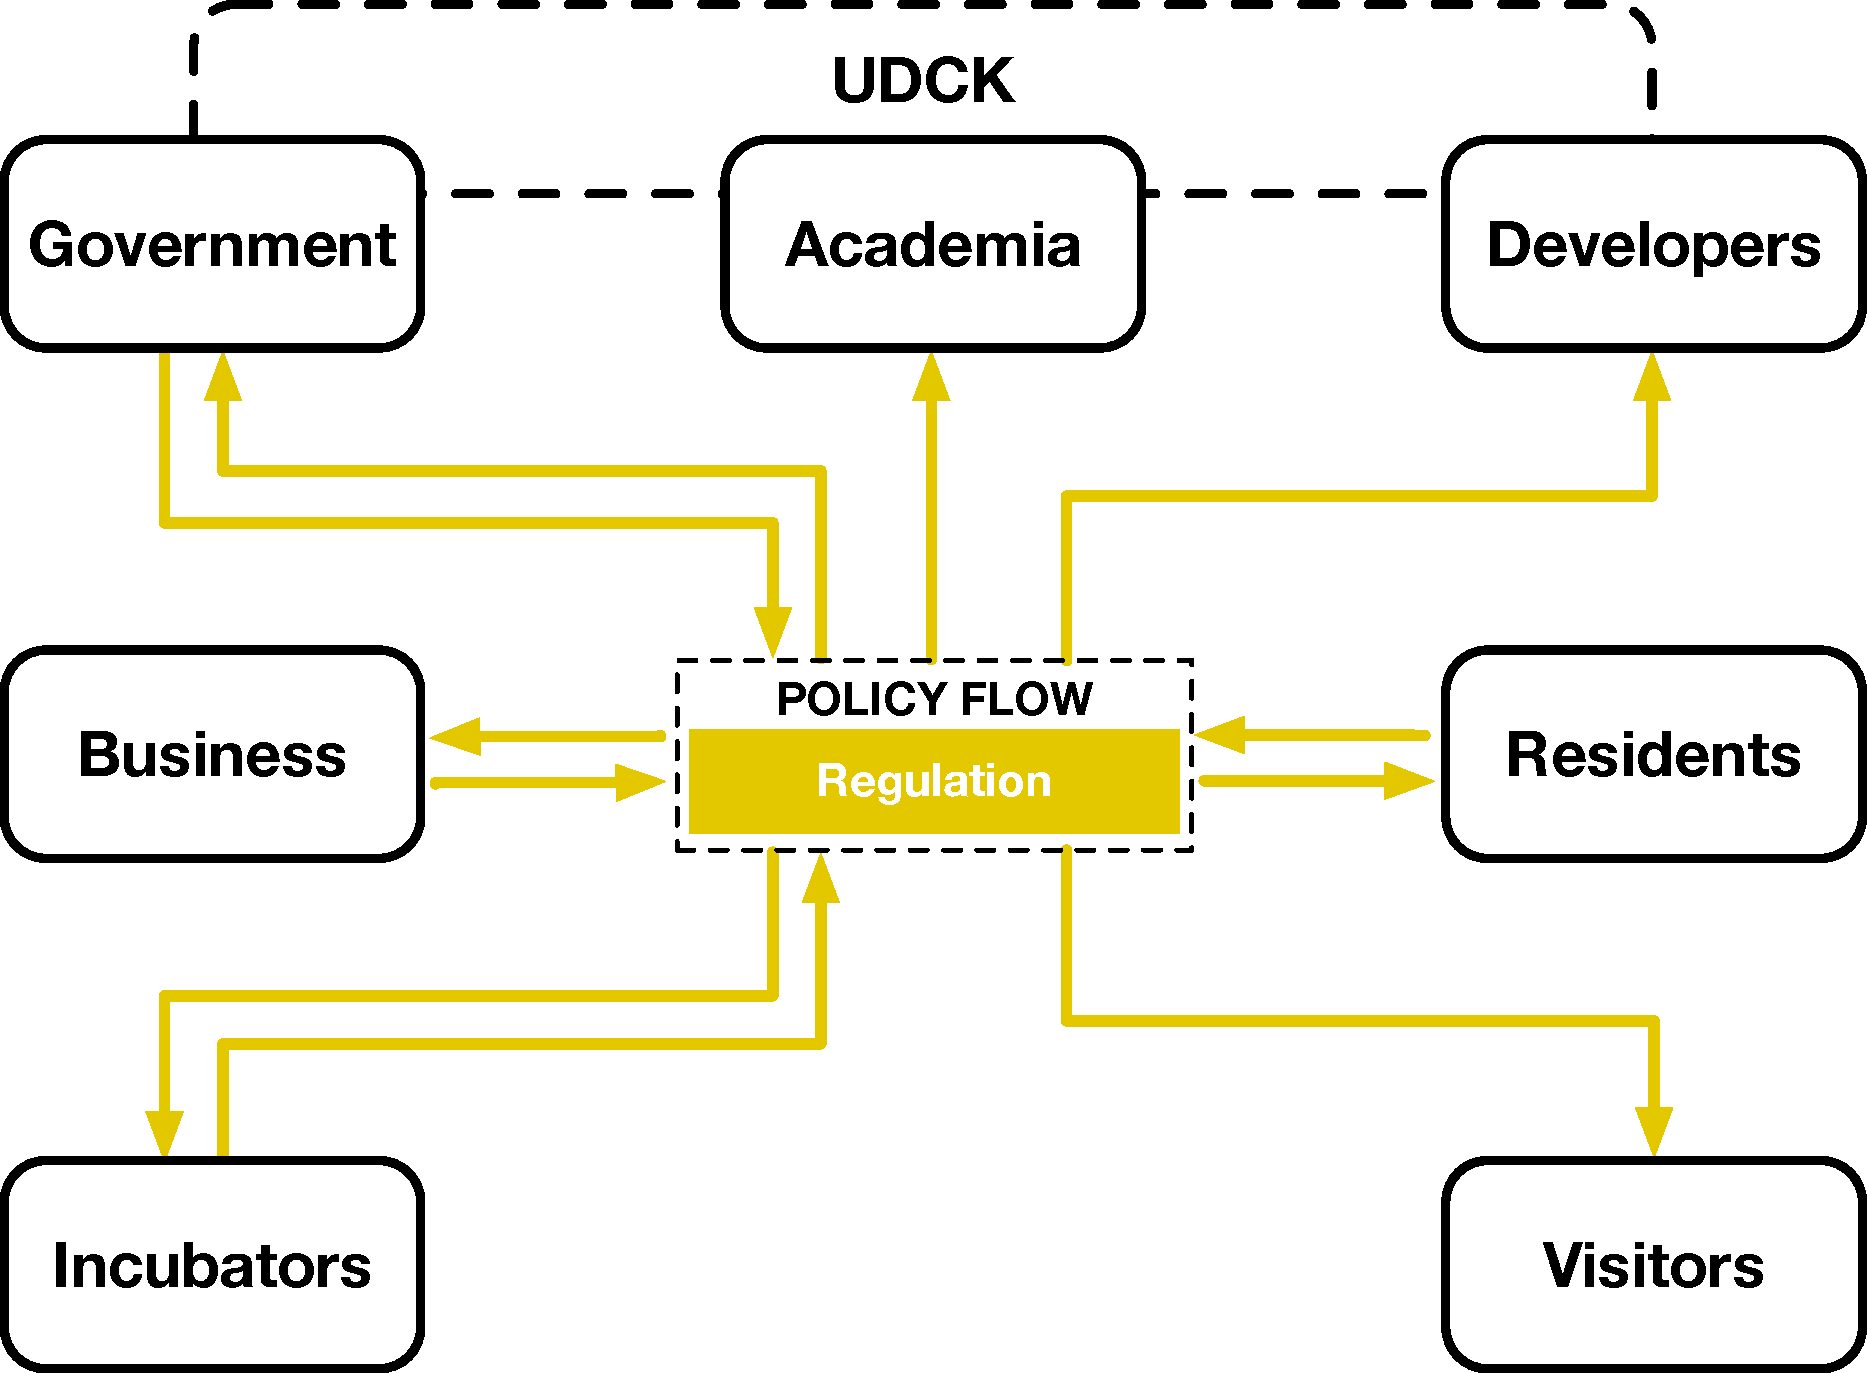
\includegraphics[width=2.5in]{SVN_3_v_6.pdf}
\caption{SVN for stakeholders of the Kashiwa-no-ha Smart City: regulation value flows added as a proposal for strengthening stakeholder relationships and leading to more successful implementation of the smart city strategy.}
\label{Compare_S}
\end{figure}

There is a clear difference between the improved model and the original model, which is reflected in the change in regulation value flow. For practical needs voiced by business, residents, and incubators, the government can respond, provide solutions, and better implement strategies through UDCK.

% ==================
% # IV. Discussion #
% ==================

\section{\textbf{Discussion}}

Previous studies suggest that a transdisciplinary approach can solve the problems traditionally found in governance with a top-down approach. Bodin et al. (2016) argue that if sustainability is the goal, collaborative governance systems are required to tackle complex problems \cite{bodin2016theorizing}. One such system is the  ``living lab'', a co-creation concept where users in a real-life environment drive innovation, encompassing social and technical dimensions simultaneously in a business-citizen-government-academia partnership. An example of a living lab described by Bergvall-K{\aa}reborn and St{\aa}hlbr{\"o}st (2009) is Botnia Living Lab, an environment for development of IT services and products where users are involved as equal co-creators along with the other stakeholders (companies, academia, and authorities) \cite{bergvall2009living}. Openness, realism, and empowerment are key concepts of the living lab. This is particularly useful in application to Kashiwa-no-ha, where stakeholder engagement is a goal, but that goal has not been fully realized.

In the living lab, users are enabled to create value. Likelihood of project success is increased, as users/beneficiaries are included and able to communicate their needs throughout the development process \cite{pallot2010living}. Smart city need not be understood as a top-down approach, but a living ``system of systems'', consisting of many stakeholders and values that work together \cite{cosgrave2013living}. To promote innovation, a stated goal of the Kashiwa-no-ha Smart City project, stakeholders need to be enabled by the development team (through UDCK) to generate and share ideas.

To strengthen the relationship between these stakeholders and UDCK, and represent this bottom-up decision-making approach, feedback regulation flows are added to the SVN flowing from residents, business, and incubators to government. Enabling good information flow between stakeholders ensures continuous feedback regarding both suitability of strategy to address stakeholder needs (reducing likelihood of emergence of problems) and progress of implementation of strategy (reducing the gap between strategy and implementation).

Lack of cultural identity is considered to be a typical case of a socio-technical problem in smart cities. Songdo in South Korea has become an innovative laboratory for policymakers and advanced technology \cite{carvalho2011urban}, but is described as a city without soul, with little room left for ordinary people to participate \cite{hollands2015critical}. In smart cities built from scratch, the emergence of a lack of cultural identity is inevitable. This is because it is difficult for residents who have moved into a smart city to form a stable social communication structure, and there is little cooperation between service providers and beneficiaries (including visitors).
 
To reduce the distance between beneficiaries and service providers, a concept like a pathway tour through the city was proposed by one of the five groups (Fig. 4). This could make the city more inclusive, strengthening social interaction between residents and visitors, helping establish cultural identity within the smart city.

\begin{figure}[ht!] %!t
\centering
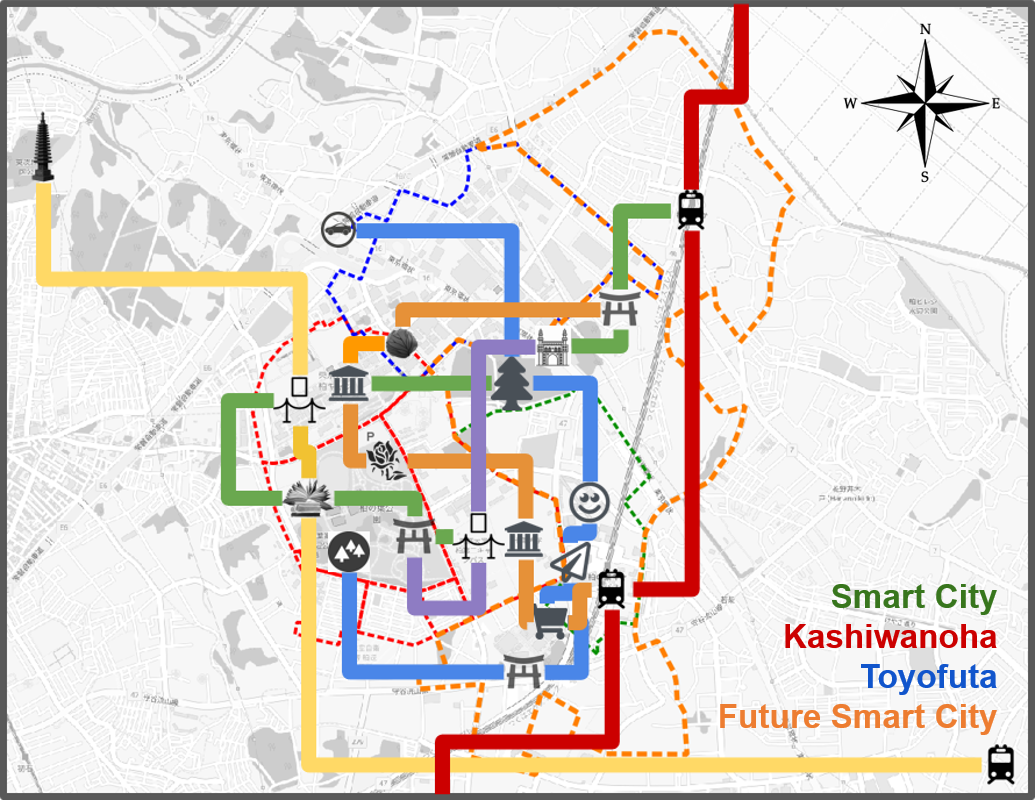
\includegraphics[width=3in]{PT.png}
\caption{A conceptual pathway tour to strengthen the relationship between service beneficiaries and providers. Proposal by the  team focused on socio-technical issues (2) lack of cultural identity.}
\label{Compare_S}
\end{figure}

% ==================
% # V. Conclusion #
% ==================

\section{\textbf{Conclusion}}

Kashiwa-no-ha Smart City maintains goals for sustainable development and has developed a strategy to achieve these goals. The implementation of this strategy has resulted in the establishment of UDCK, a platform overseen by a public-private-academic partnership to facilitate smart city stakeholder collaboration. Despite the creation of a strategy to promote the sustainable development of Kashiwa-no-ha, newly emerging socio-technical problems can be found, indicating implementation of the strategy has not been completely successful.

Based on the above findings and discussion, we conclude that some stakeholders (residents, businesses, incubators) are not adequately connected in Kashiwa-no-ha, despite the presence of UDCK. By utilising a transdisciplinary concept like ``living lab'', bottom-up stakeholder collaboration can be facilitated to ensure services provided align with stakeholder needs, bridging the gap between strategy and implementation, and reducing the strain of socio-technical problems.

% ==================
% # ACKNOLEDGMENTS #
% ==================

% use section* for acknowledgement

\section*{\textbf{Acknowledgment}}

% We would like to express our sincere appreciation to all the student collaborators of GFE Kashiwa-no-ha 2017-18 who, with the authors, produced the research results that this paper is based upon.

We would like to express our sincere appreciation to all the student collaborators of GFE Kashiwa-no-ha 2017-18 who, with the authors, produced the research results that this paper is based upon.

% ==============
% # REFERENCES #
% ==============

\bibliographystyle{IEEEtran}
\bibliography{IEEEabrv,biblio_traps_dynamics}

\end{document}